\documentclass{scrartcl}
\usepackage[utf8]{inputenc}
\usepackage{hyperref}
\usepackage{url}
\usepackage{natbib}
\usepackage{graphicx}
\usepackage{cleveref} % this must be the last package to be loaded

\newcommand{\emailaddr}[1]{\href{mailto:#1}{\texttt{#1}}}

\title{\LARGE
  Final Report\\
    Distributed File Hosting
}
\subtitle{Final Report for the Distributed Systems Course 2025/2026}

% Consider watching:
% https://www.youtube.com/watch?v=ihxSUsJB_14
% https://www.youtube.com/watch?v=XTFWaV55uDo

\author{
    Andrea Alfonsi \\ \emailaddr{andrea.alfonsi3@studio.unibo.it}
}

\date{\today}

\begin{document}

\maketitle

\begin{abstract}
This report presents a lightweight distributed file hosting system implemented in Python using FastAPI and asyncio. The system is composed of multiple peer nodes, each exposing a REST API for client operations and a TCP JSON-RPC channel for internal coordination. Files are replicated across nodes with configurable replication and quorum parameters. Each write is versioned with Lamport logical clocks, and conflicts are deterministically resolved using the tuple $(lamport\_counter, version\_node)$. A periodic health monitor detects peer failures and triggers recovery synchronization when nodes rejoin.

The implementation targets a practical balance between availability and consistency in partitioned environments. Write operations succeed when the configured write quorum is reached, while temporary divergence is repaired through background anti-entropy. The project includes containerized deployment through Docker Compose (three-node topology), a reproducible simulation script for failure and recovery scenarios, and a documented user workflow for upload, download, monitoring, and resilience validation.
\end{abstract}

\section*{Disclaimer (if needed)}

During the preparation of this work, the author used GitHub Copilot to improve wording quality and structure of the report.

After using this tool, the author reviewed and edited the generated text as needed and takes full responsibility for the final content.

\section{Concept}\label{concept}

The developed product is a distributed web service for file hosting. Each node provides a REST interface for client-facing upload, listing, metadata inspection, and download. Nodes also run an internal RPC service to replicate data, exchange metadata catalogs, and recover after failures.

The system is designed to handle frequent uploads of small and medium files, occasional downloads from any reachable node, and operational health checks of cluster status. It is also suited for fault-injection experiments in teaching or testing scenarios.

Distribution is motivated by three main concerns. First, \textbf{fault tolerance}: files are replicated across peers, so node crashes do not imply immediate data loss. Second, \textbf{availability}: client requests can be served by multiple nodes, and writes can still complete as long as quorum is met. Third, \textbf{resource sharing}: storage and traffic are spread across nodes, avoiding a single point of congestion.

\section{Requirements Elicitation and Analysis}\label{requirements}

\subsection*{Glossary}
\begin{itemize}
  \item \textbf{Logical path}: user-visible path used to identify a file in the system (for example, \texttt{docs/report.pdf}).
  \item \textbf{Replica}: copy of a file stored on a different node.
  \item \textbf{Write quorum}: minimum number of acknowledgements required for a successful write.
  \item \textbf{Catalog}: node metadata map from logical path to file metadata and version.
\end{itemize}

\subsection*{Functional requirements}
\begin{description}
  \item[FR1 -- File upload] A client shall upload a file with an optional logical path through a REST endpoint.
  \textbf{Acceptance criterion:} A \texttt{POST /files/upload} request returns HTTP 201 with metadata when quorum is reached.

  \item[FR2 -- File download] A client shall download the most recent file version from any node.
  \textbf{Acceptance criterion:} \texttt{GET /files/\{logical\_path\}/download} returns HTTP 200 and file bytes for existing files.

  \item[FR3 -- Metadata inspection] A client shall list node metadata and inspect per-file metadata.
  \textbf{Acceptance criterion:} \texttt{GET /files} and \texttt{GET /files/\{logical\_path\}/metadata} return JSON metadata when available.

  \item[FR4 -- Replication] On successful upload, the ingress node shall replicate to selected peers.
  \textbf{Acceptance criterion:} The upload response includes replica targets and acknowledged replicas.

  \item[FR5 -- Recovery synchronization] A node that becomes reachable again shall be synchronized automatically.
  \textbf{Acceptance criterion:} After restart of a failed node, it eventually serves the latest uploaded version.

  \item[FR6 -- Health visibility] Operators shall inspect node and peer health status.
  \textbf{Acceptance criterion:} \texttt{GET /health} reports node id, clock, quorum settings, and peer reachability.
\end{description}

\subsection*{Non-functional requirements}
\begin{description}
  \item[NFR1 -- Deterministic conflict handling] Concurrent versions shall be resolved consistently.
  \textbf{Acceptance criterion:} Version comparison based on $(lamport\_counter, version\_node)$ produces deterministic winners.

  \item[NFR2 -- Availability under partial failures] Write operations should continue while enough replicas are reachable.
  \textbf{Acceptance criterion:} With replication factor 3 and write quorum 2, writes succeed when at least one peer acknowledges.

  \item[NFR3 -- Bounded failure detection] Peer liveness checks shall run periodically.
  \textbf{Acceptance criterion:} Reachability state changes appear in health output after at most one monitoring period plus RPC timeout.

  \item[NFR4 -- Durability per node] Stored file bytes and metadata shall survive process restarts.
  \textbf{Acceptance criterion:} Restarting a container preserves files and metadata in mounted volumes.
\end{description}

\subsection*{Implementation constraints}
\begin{description}
  \item[IR1 -- Language/runtime] The system shall use Python 3.12 to align with course tooling and team familiarity.
  \textbf{Acceptance criterion:} The project runs in the provided Python 3.12 Docker image.

  \item[IR2 -- Deployment] The project shall be runnable with Docker Compose for reproducible evaluation.
  \textbf{Acceptance criterion:} A single \texttt{docker compose up -d --build} command starts the three-node cluster.

  \item[IR3 -- HTTP interface] Client-facing operations shall be exposed via REST/HTTP.
  \textbf{Acceptance criterion:} Upload, download, list, metadata, and health endpoints are callable through standard HTTP clients.
\end{description}

\subsection{Relevant Distributed System Features}
\label{ds-features}

Transparency is partially relevant: clients can use any node through the same REST API, but distribution details are intentionally visible in health and replication diagnostics. Fault tolerance and dependability are central goals, addressed through replication, periodic ping checks, and post-failure synchronization. Scalability is moderately relevant: the peer-based architecture is horizontally extensible, but no dynamic membership or sharding is implemented in the current version.

Security is currently limited, as no authentication or authorization layer is present; this is acceptable for a lab prototype but not production-ready. Resource sharing is highly relevant, since storage is distributed across nodes through replication and metadata coordination. Communication uses standard HTTP and JSON, ensuring openness and interoperability with external clients.

Components are modular --- config, storage, RPC, and cluster logic --- which supports evolvability and maintainability. Performance and concurrency are addressed through async I/O and parallel replication, with the design prioritizing simplicity over peak throughput. Finally, the stack is lightweight and containerized, minimizing infrastructure and onboarding costs.

\section{Design}\label{design}

The design follows a symmetric peer-node architecture. Each node can receive client writes, store local data, replicate updates, and answer reads. This removes a single leader dependency and supports availability under partial failures.

In the taxonomy of distributed systems, this structure is classified as a \textbf{peer-to-peer} architecture: all participants are functionally equivalent and no central coordinator mediates interactions. Compared to client-server or hierarchical designs, the symmetric topology eliminates the need for a leader election protocol, but places full responsibility for conflict resolution on the version ordering mechanism shared across all nodes.

\subsection{Architecture}\label{architecture}

The adopted style is \textbf{service-based peer-to-peer replication with dual interfaces}. Externally, nodes expose a REST/HTTP API for client operations; internally, they communicate over a TCP JSON-RPC channel for coordination tasks such as ping, catalog exchange, metadata and content fetch, and file replication. This split keeps the client interface simple while allowing richer internal protocols.

The component-level view is shown in \cref{fig:component-view}.

\begin{figure}
  \centering
  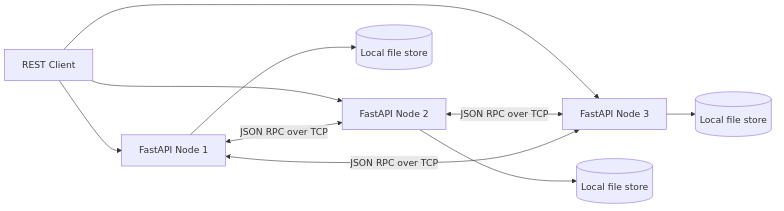
\includegraphics[width=0.95\textwidth]{figures/component-view.png}
  \caption{Component view of the distributed file hosting system}
  \label{fig:component-view}
\end{figure}

\subsection{Infrastructure}\label{infrastructure}

The cluster consists of three identical node services and any number of REST clients. Each node exposes a REST endpoint on port 8000, mapped to host ports 8001, 8002, and 8003, along with an RPC endpoint on port 9000, mapped to host ports 9001, 9002, and 9003. Persistent storage is provided through a dedicated named volume per node, containing file blobs and a \texttt{metadata.json} document. All nodes run within a shared Docker Compose network for local deployment, and the same design can be mapped to separate physical or virtual hosts. Peer addresses are communicated through the static \texttt{PEERS} environment variable, which holds a JSON array of host and port configurations.

File placement across the cluster reflects a key concern of computing with space in distributed systems: rather than replicating all files to all nodes, each file has a defined set of responsible replicas determined by hashing its logical path and rotating through the sorted peer list. This makes placement deterministic and stable for a fixed cluster topology, distributing storage load without requiring a central directory or a coordination round on every upload.

\subsection{Modelling}\label{modelling}

The main domain entities are \texttt{PeerConfig}, \texttt{FileVersion}, \texttt{FileMetadata}, and logical file content. Each node stores file bytes under a deterministic local filename and indexes metadata by logical path. The system recognizes five domain events: file uploaded, file replicated, peer failed, peer recovered, and catalog synchronized. Messages fall into two categories: REST commands (upload, download, list) and RPC commands (ping, replicate\_file, get\_file\_metadata, get\_file\_content, get\_catalog). System state at any point is defined by the local metadata catalog, the blob storage contents, the current Lamport clock value, and the per-peer reachability map.

\subsection{Interaction}\label{interaction}

On the upload path, a client sends a file to any node; that node writes locally and replicates the content in parallel to selected peers. A response is returned as successful only if the write quorum is reached. On the read path, a node compares its local metadata with peer metadata and fetches content from the newest source when needed. A background monitoring task periodically pings each known peer and updates their reachability status accordingly. When a peer transitions from unreachable to reachable, a two-way synchronization is triggered to repair stale or missing data. The overall pattern combines request/response interactions with periodic anti-entropy synchronization.

The upload interaction is detailed in \cref{fig:upload-flow}; recovery synchronization is illustrated in \cref{fig:recovery-flow}.

\begin{figure}
  \centering
  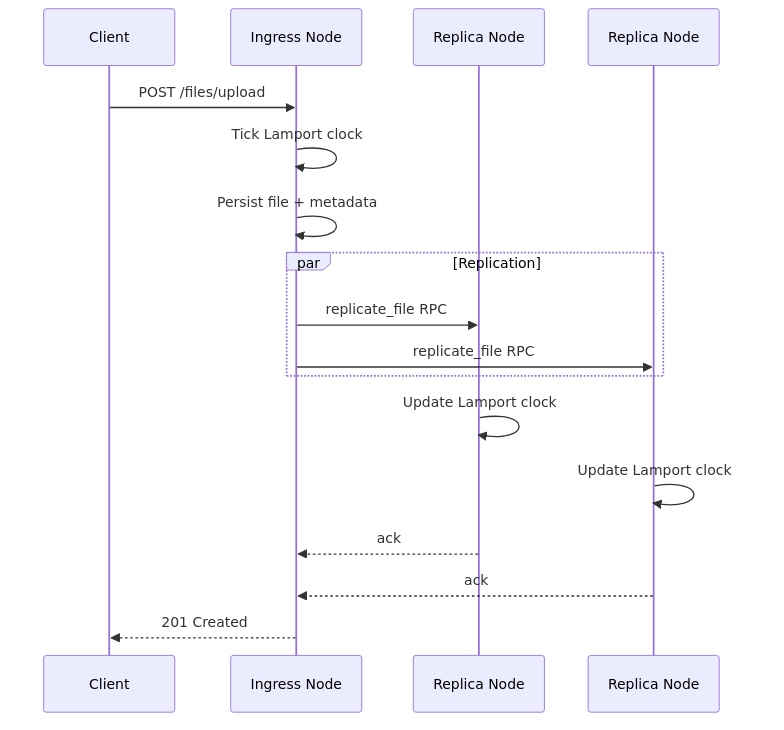
\includegraphics[width=0.98\textwidth]{figures/upload-flow.png}
  \caption{Sequence of a client upload with parallel replication}
  \label{fig:upload-flow}
\end{figure}

\begin{figure}
  \centering
  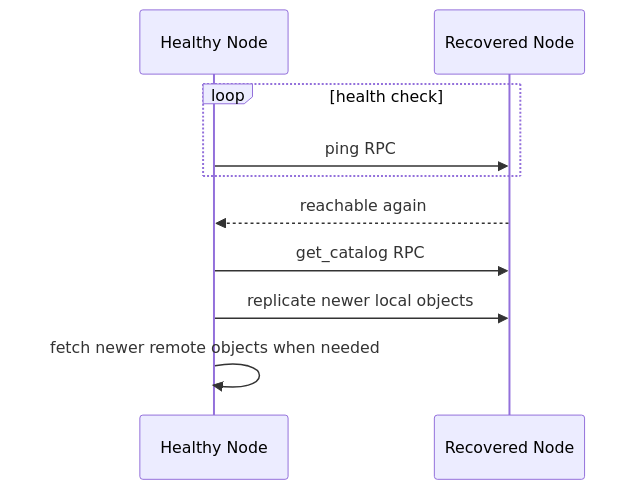
\includegraphics[width=0.98\textwidth]{figures/recovery-flow.png}
  \caption{Sequence of peer recovery and catalog-based synchronization}
  \label{fig:recovery-flow}
\end{figure}

\subsection{Behaviour}\label{behaviour}

Nodes are stateful components: each one manages local storage, metadata, peer status, and a Lamport clock. On upload, the ingress node updates its state by ticking the clock, creating a new file version, and persisting the content. When a \texttt{replicate\_file} RPC message arrives, a replica node updates its state using Lamport update semantics. The storage layer accepts a new version only if it is strictly newer than the currently stored one, preventing regressions. Recovery logic can both push locally newer files to a rejoined peer and pull newer remote files from it.

The use of Lamport logical clocks reflects a core result from the theory of distributed computation: in a network of processes communicating solely by message passing, it is impossible to synchronise physical clocks to arbitrary precision, making a shared global time reference unavailable. Lamport's \emph{happened-before} relation ($\rightarrow$) defines a partial causal order on events --- if event $a$ causes event $b$ then $C(a) < C(b)$ --- and the update rule $C_j \leftarrow \max(C_j, C_i) + 1$ on message receipt propagates this ordering across nodes. The version tuple $(lamport\_counter, version\_node)$ extends this partial order to a strict total order by appending the originating node identifier as a deterministic tie-breaker, ensuring every node independently agrees on the winning version of a file without additional coordination.

\subsection{Data and Consistency Issues}\label{data-and-consistency-issues}

Persistent data includes file bytes and metadata fields such as path, size, checksum, MIME type, and version information. The storage model relies on the filesystem for blobs and on a per-node \texttt{metadata.json} document for indexed metadata; no external DBMS is used. Queries are local map lookups and catalog exchanges. Concurrent operations within a node are protected with thread locks in the clock and storage classes. Metadata versions and file content are the shared cross-node data, transported over RPC during replication and recovery. The consistency model is eventual consistency with deterministic last-writer-wins ordering based on Lamport metadata tuples.

The system's positioning is best understood through the CAP theorem, which establishes that a distributed system cannot simultaneously guarantee all three of the following properties: \emph{consistency} (every read returns the most recent write), \emph{availability} (every request receives a response), and \emph{partition tolerance} (the system continues operating despite network splits). The system deliberately prioritises \textbf{availability and partition tolerance}: under a network partition, nodes that can reach write quorum continue accepting writes, while minority nodes reject them. The resulting temporary divergence is bounded and resolved deterministically once connectivity is restored, classifying the system as \emph{eventually consistent}.

The replication model is leaderless and optimistic: any node can accept writes and propagate them to replicas without a designated primary. This avoids the single-point bottleneck and leader election overhead of primary-backup replication, but transfers the responsibility for convergence entirely to the version ordering mechanism.

\subsection{Fault-Tolerance}\label{fault-tolerance}

Replication is configurable through a replication factor; replica targets are selected by hashing the logical path and rotating through the peer list. Liveness is monitored through periodic \texttt{ping} RPC checks, with a timeout enforced on every RPC operation. If the number of write acknowledgements falls below quorum, the node returns an error to the client rather than silently accepting an under-replicated write. When a peer rejoins the cluster, background synchronization repairs stale or missing data. Errors occurring during replication or recovery are isolated per peer and logged without crashing the node.

The fault-tolerance strategy maps to the four classical dependability attributes: \emph{availability} (requests are served even when peers have crashed), \emph{reliability} (data written to quorum survives single-node failures), \emph{safety} (writes are rejected rather than silently accepted when quorum cannot be reached), and \emph{maintainability} (rejoining nodes are repaired automatically without operator intervention). The assumed failure model is crash-stop: nodes either operate correctly or stop responding entirely. Byzantine failures --- where a node sends incorrect or malicious messages --- are outside the scope of this prototype.

Write quorum acts as a lightweight substitute for full consensus. Protocols such as Paxos and Raft guarantee that all replicas agree on a single value before any client receives a success response, providing linearisable consistency at the cost of higher latency and synchronisation overhead. The quorum approach relaxes this guarantee: only $W$ of $N$ nodes need to acknowledge a write, and for the default three-node topology with $W = 2$ the system tolerates one node failure without blocking writes. The trade-off is that two concurrent writes issued to opposite sides of a partition can both succeed and be reconciled by last-writer-wins after reconnection, rather than one being rejected outright.

The per-node \texttt{metadata.json} document functions as a durable checkpoint of the node's distributed catalog view. On recovery, the synchronization procedure performs a catalog diff --- analogous to replaying a write-ahead log from the last known checkpoint --- to identify missing or outdated entries and restore the node to a consistent state. Only files that are actually stale are transferred, minimising recovery bandwidth.

\subsection{Availability}\label{availability}

No dedicated cache layer or explicit load balancer is included; clients may freely choose any node endpoint. Under a network partition, the system remains writable as long as the write quorum can be reached among the surviving nodes. Divergent replicas are reconciled when connectivity is restored through catalog-based synchronization.

\subsection{Security}\label{security}

The current prototype does not implement authentication, authorization, or transport encryption. Integrity is partially supported through SHA-256 checksums stored in file metadata. Security hardening is addressed in \cref{future-works}.

\section{Implementation}\label{implementation}

The system uses HTTP as the client-facing protocol and raw TCP for internal node-to-node RPC. Payloads are represented in JSON for both REST and RPC; file content is encoded in Base64 for transport over the RPC channel. Persistence relies on direct filesystem and JSON document handling, with no SQL or NoSQL engine involved. Authentication and authorization are not yet implemented in this iteration.

\subsection{Technological details}\label{technological-details}

The runtime is Python 3.12. FastAPI provides the REST framework and Uvicorn serves as the ASGI server. Concurrency is handled through asyncio, which underpins parallel replication, peer monitoring, and RPC operations. Deployment is managed with Docker and Docker Compose, providing a reproducible three-node environment.

The codebase is organized into five main modules. \texttt{cluster.py} handles orchestration, quorum logic, replication, and recovery. \texttt{storage.py} manages persistent metadata and blob storage. \texttt{rpc.py} implements line-delimited JSON-RPC over TCP. \texttt{lamport.py} encapsulates logical clock semantics. \texttt{main.py} defines REST endpoints and controls the application lifecycle.

\section{Validation}\label{validation}

\subsection{Automatic Testing}\label{automatic-testing}

Dedicated unit tests are not present in this iteration. Integration and end-to-end behavior are instead exercised automatically by \texttt{scripts/simulate\_cluster.py}. The script covers the following scenario: it starts the cluster, uploads a first file version, verifies that a replica node can serve it, stops one node, uploads a second version during the simulated failure, restarts the stopped node, and then verifies that the recovered node serves the latest version. The automated scenario can be run with \texttt{python3 scripts/simulate\_cluster.py}.

In terms of requirement coverage, the script exercises FR1, FR2, and FR4 through upload and read checks; FR5 through post-restart synchronization verification; and NFR2 through a quorum-based write with one node down.

\subsection{Acceptance test}\label{acceptance-test}

Manual acceptance testing was performed through \texttt{curl} commands against all node endpoints. The tested behaviors included upload with metadata inspection, cross-node file download, health endpoint changes observed after stopping and restarting containers, and write failure behavior when the quorum could not be reached. Manual checks were particularly useful for inspecting response payloads and operational diagnostics interactively.

\section{Deployment}\label{deployment}

The only required software is Docker Engine with Docker Compose support. The entire cluster is started with:
\begin{verbatim}
docker compose up -d --build
\end{verbatim}
After startup, three containers are running and accessible on REST ports 8001, 8002, and 8003. Each container is configured with its node identity, port assignments, data directory, quorum parameters, peer list, and RPC timeout through environment variables. Persistent storage is provided by the named volumes \texttt{node1-data}, \texttt{node2-data}, and \texttt{node3-data}, which survive container restarts. A standalone local run is also possible without containers by using a virtual environment and launching Uvicorn directly, with distinct environment variables set for each node.

\section{User Guide}\label{user-guide}

Start the cluster by running:
\begin{verbatim}
docker compose up -d --build
\end{verbatim}

To upload a file, send a multipart POST request with the file content and an optional logical path:
\begin{verbatim}
curl -X POST http://127.0.0.1:8001/files/upload \
  -F "file=@./sample.txt" \
  -F "logical_path=docs/sample.txt"
\end{verbatim}

To list the metadata catalog on a node:
\begin{verbatim}
curl http://127.0.0.1:8001/files
\end{verbatim}

To download the file from a different node:
\begin{verbatim}
curl http://127.0.0.1:8002/files/docs/sample.txt/download -o sample.txt
\end{verbatim}

To inspect cluster health:
\begin{verbatim}
curl http://127.0.0.1:8001/health
\end{verbatim}

To run the full failure and recovery demonstration:
\begin{verbatim}
python3 scripts/simulate_cluster.py
\end{verbatim}

\section{Self-evaluation}\label{self-evaluation}

\textbf{Role and contribution.} I designed and implemented the full prototype, including the API layer, replication logic, Lamport clock management, persistence layer, containerized deployment, and demonstration script.

The main strengths of the project are its clear modular separation of concerns, a reproducible deployment requiring minimal setup, practical failure handling with automatic recovery, and deterministic version resolution in distributed update scenarios.

On the other hand, several weaknesses remain. The system lacks a security layer covering authentication, authorization, and TLS. Automated testing is limited in depth, with no unit test suite in place. Peer configuration is static and no dynamic membership mechanism has been implemented. Finally, no explicit load balancing or advanced placement policies are currently supported.

\section{Future works}\label{future-works}

Several improvements are planned for future iterations. On the security front, the priority is to introduce authentication and authorization --- for example, JWT tokens with role-based policies --- and to enable TLS for both REST and RPC channels. Testing coverage should be extended with comprehensive unit and integration test suites backed by CI automation.

The cluster management layer would benefit from dynamic node membership and service discovery, removing the current dependency on static configuration. Consistency semantics could be strengthened with tunable read-repair and optional vector clocks. Operational visibility is another planned improvement, with Prometheus-compatible telemetry as a first step. Finally, the data model could be extended with deletion semantics, tombstones, and configurable retention policies, and explicit load balancing and request routing strategies could be introduced.

\bibliographystyle{plain}
\nocite{*}
\bibliography{references}

\end{document}